%*******10********20********30********40********50********60********70********80
\clearpage
\subsection{Reactive Aggregate Ratio Related to Behavior of Concrete During ASR Expansion}

In this section, the relationship between ASR reactive aggregate ratio and behavior during expansion is discussed.

Expansion simulation result of 30\% coarse aggregate model is used here, and different ASR reactive ratio (25\% of total coarse aggregate and 75\% of total coarse aggregate) is given (Figure \ref{fig:Aggregate_Percentagedsfsdf}), to analyze how the change in ASR reactive aggregate percentage influence the cracking pattern.

\begin{figure}[!h]
\centering
\begin{subfigure}{.5\textwidth}
  \centering
  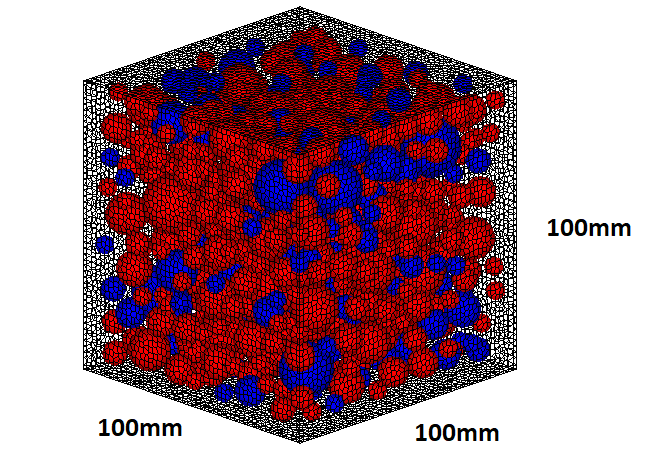
\includegraphics[width=.8\linewidth]{Files/Aggregate/A30P75.png}%FIXME
  \caption{30\% Coarse Aggregate with 75\% ASR Reactive Aggregate}
  \label{fig:A15_model}
\end{subfigure}%
\begin{subfigure}{.5\textwidth}
  \centering
  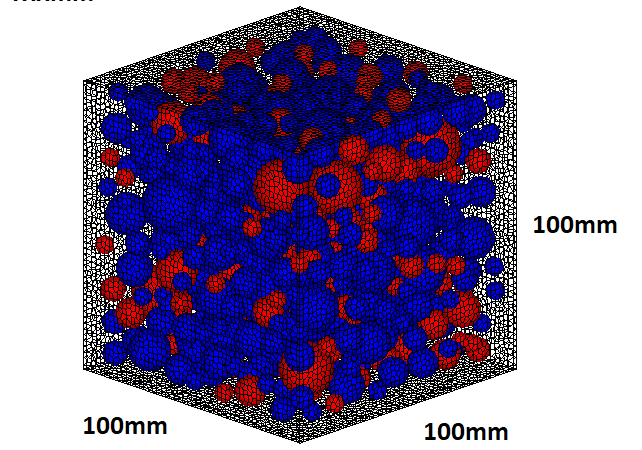
\includegraphics[width=.8\linewidth]{Files/Aggregate/A30P25.png} %FIXME
  \caption{30\% Coarse Aggregate with 25\% ASR Reactive Aggregate}
  \label{fig:A15_model}
\end{subfigure}
\caption{25\% and 75\% ASR Reactive Aggregate Ratio Model}
\label{fig:Aggregate_Percentagedsfsdf}
\end{figure}

Table \ref{table:A30P25vsA30P75_EXP} summarized the giving initial strain in each step and the total step of expansion giving in the two models compared in this section. Relatively larger initial strains are given to the less ASR reactive coarse aggregate cases (25\% ASR reactive aggregate cases here) to reach relatively closer global expansion ratio for comparing.

\begin{table}[ht!]
  \caption{One Dimensional Expansion Ratio[\%] in A30P25 and A30P25 ASR Expansion Simulation}
\centering
\begin{tabular}{ ||p{2cm}|p{2cm}|p{2cm}|p{2cm}|p{2cm}|| }
 \hline
 Aggregate Ratio[\%] &  Reactive Aggregate Ratio[\%]  & Initial Strain (Each Step) & Expanding Steps & Final Expansion [\%] \\ [0.5ex]
 \hline\hline
 30 & 75 & 0 & 0 & 0\\
 30 & 75 & 0.0002 & 20 & 0.0699\\
 30 & 75 & 0.0005 & 20 & 0.1936\\
 30 & 75 & 0.001 & 20 & 0.4223\\
 30 & 75 & 0.002 & 20 & 0.8832\\
 30 & 75 & 0.003 & 20 & 1.3224\\

 30 & 25 & 0 & 0 & 0\\
 30 & 25 & 0.001 & 20 & 0.1651\\
 30 & 25 & 0.002 & 20 & 0.3606\\
 30 & 25 & 0.004 & 20 & 0.7024\\
 30 & 25 & 0.006 & 20 & 1.0201\\
 \hline
\end{tabular}

\label{table:A30P25vsA30P75_EXP}
\end{table}

%TODO: plot {table:A30P25vsA30P75_EXP}


\begin{figure}[!h]
\centering

    %*******
    \begin{subfigure}{.5\textwidth}
      \centering
      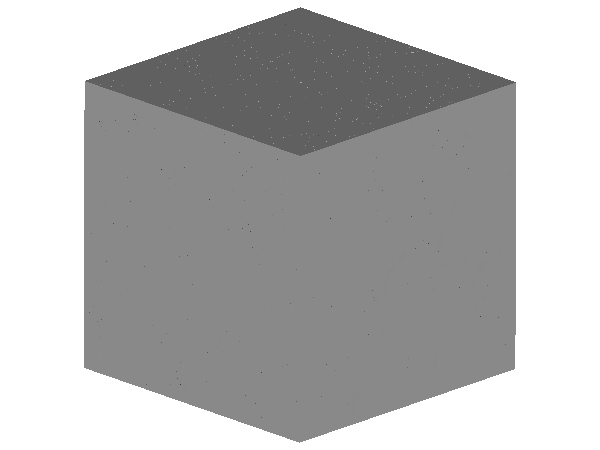
\includegraphics[width=.8\linewidth]{Files/exp_3D/ASR/A30Undamaged.png} %TODO: Fix. Should be A15
    \caption{Case 0: 0\% Expansion}
    \end{subfigure}%
    %*******
    \begin{subfigure}{.5\textwidth}
      \centering
      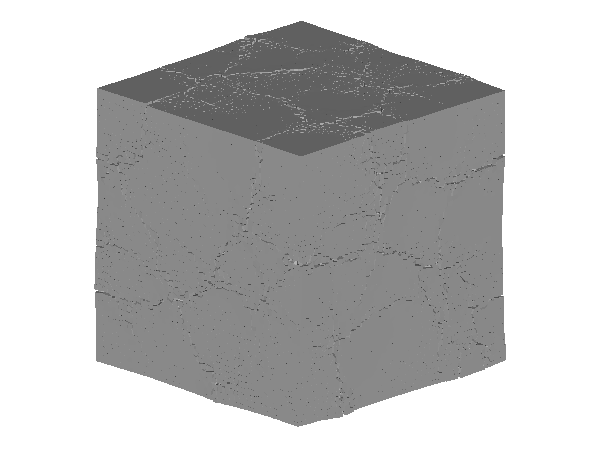
\includegraphics[width=.8\linewidth]{Files/exp_3D/ASR/A30P25_1_3d.png}
    \caption{Case 1: 0.1651\% Expansion}
    \end{subfigure}
    %*******
    \begin{subfigure}{.5\textwidth}
      \centering
      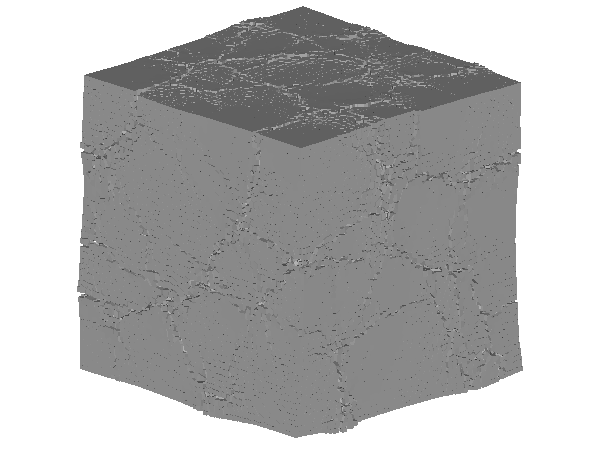
\includegraphics[width=.8\linewidth]{Files/exp_3D/ASR/A30P25_2_3d.png}
    \caption{Case 2: 0.3606\% Expansion}
    \end{subfigure}%
    %*******
    \begin{subfigure}{.5\textwidth}
      \centering
      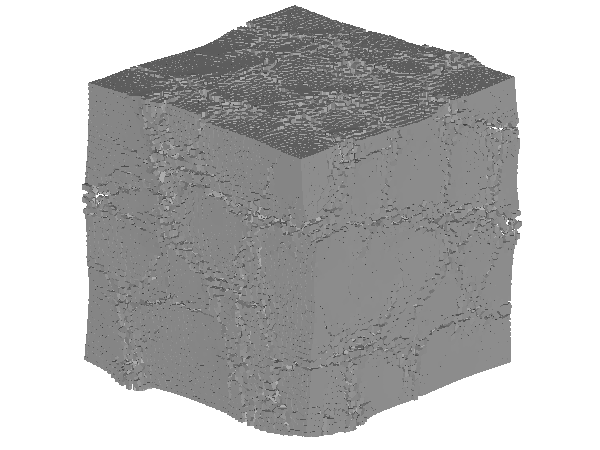
\includegraphics[width=.8\linewidth]{Files/exp_3D/ASR/A30P25_3_3d.png}
    \caption{Case 3: 0.7024\% Expansion}
    \end{subfigure}
    %*******
    \begin{subfigure}{.5\textwidth}
      \centering
      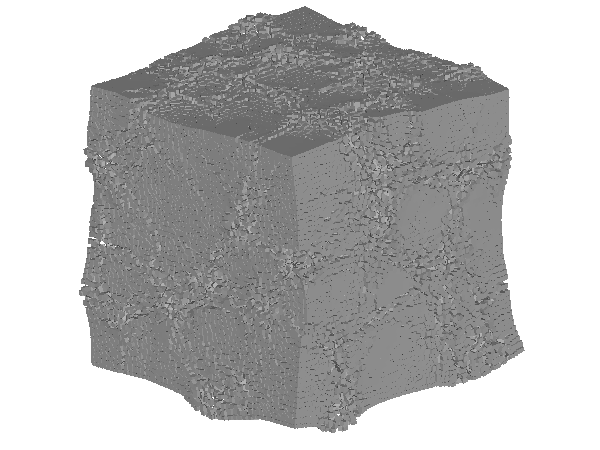
\includegraphics[width=.8\linewidth]{Files/exp_3D/ASR/A30P25_4_3d.png}
    \caption{Case 4: 1.0201\% Expansion}
    \end{subfigure}%
    %*******


  \caption{3D Surface Cracks ($Deformation \times 10$)}
  \label{fig:ASR_A30P25_3D}
\end{figure}

% Surface of one side
\begin{figure}[!h]
\centering

    %*******
    \begin{subfigure}{.5\textwidth}
      \centering
      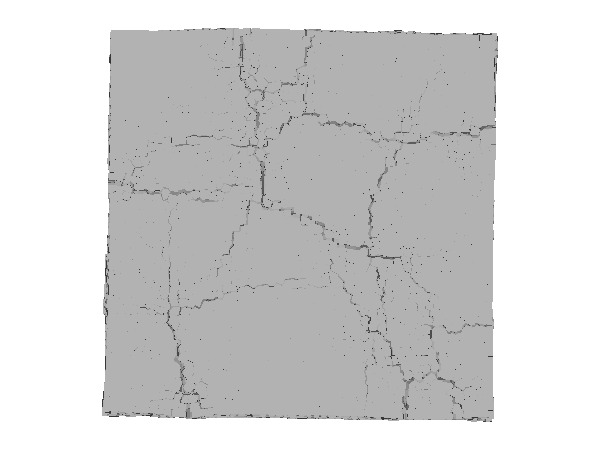
\includegraphics[width=.8\linewidth]{Files/exp_3D/ASR/A30P25_1_3ds.png}
    \caption{Case 0: 0\% Expansion}
    \end{subfigure}%
    %*******
    \begin{subfigure}{.5\textwidth}
      \centering
      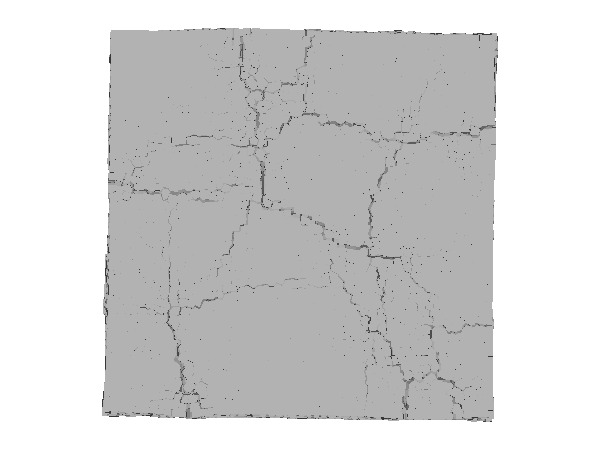
\includegraphics[width=.8\linewidth]{Files/exp_3D/ASR/A30P25_1_3ds.png}
    \caption{Case 1: 0.1651\% Expansion}
    \end{subfigure}
    %*******
    \begin{subfigure}{.5\textwidth}
      \centering
      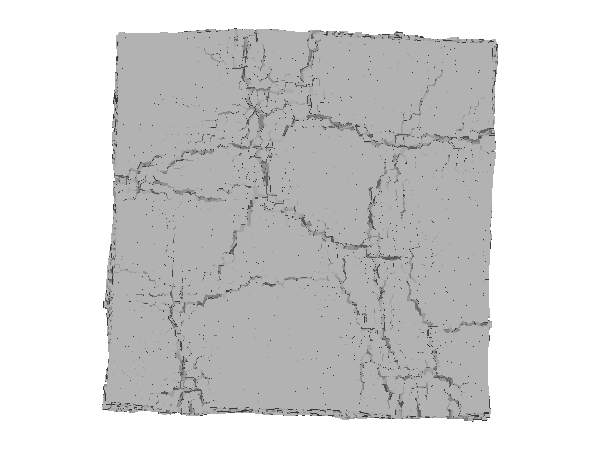
\includegraphics[width=.8\linewidth]{Files/exp_3D/ASR/A30P25_2_3ds.png}
    \caption{Case 2: 0.3606\% Expansion}
    \end{subfigure}%
    %*******
    \begin{subfigure}{.5\textwidth}
      \centering
      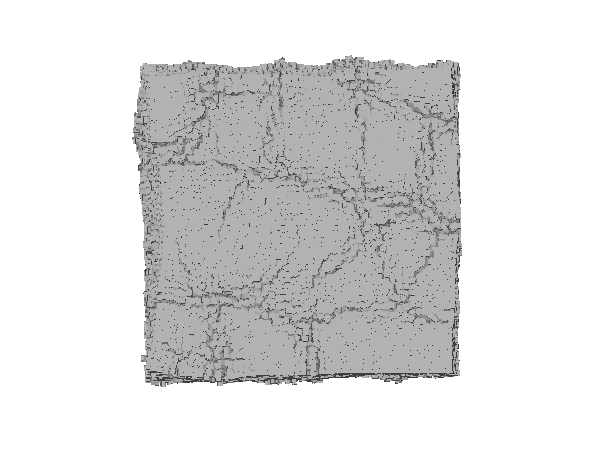
\includegraphics[width=.9\linewidth]{Files/exp_3D/ASR/A30P25_3_3ds.png}
    \caption{Case 3: 0.7024\% Expansion}
    \end{subfigure}
    %*******
    \begin{subfigure}{.5\textwidth}
      \centering
      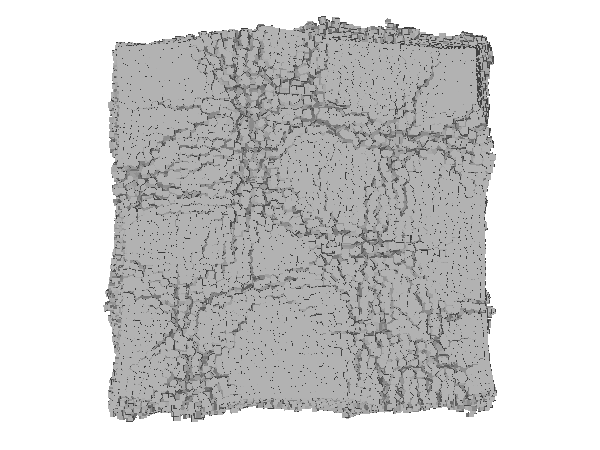
\includegraphics[width=.8\linewidth]{Files/exp_3D/ASR/A30P25_4_3ds.png}
    \caption{Case 4: 1.0201\% Expansion}
    \end{subfigure}%
    %*******

  \caption{3D Surface Cracks (Single Side View, $Deformation \times 10$)}
  \label{fig:ASR_A30P25_3DS}
\end{figure}

% 3D inner crack
\begin{figure}[!h]
\centering

    %*******
    \begin{subfigure}{.5\textwidth}
      \centering
      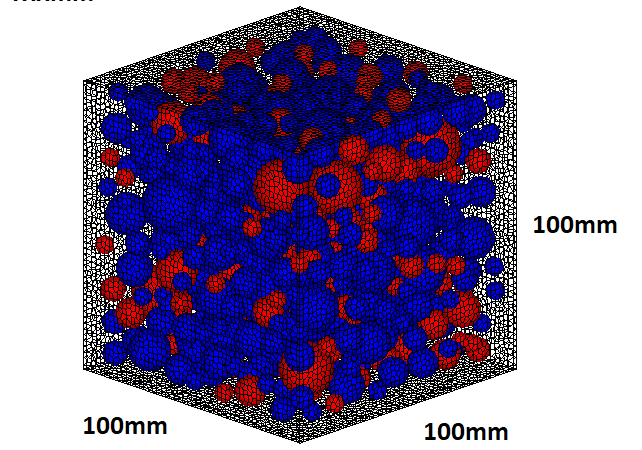
\includegraphics[width=.8\linewidth]{Files/Aggregate/A30P25.png} %TODO: Fix. Should be A15
    \caption{Case 0: 0\% Expansion}
    \end{subfigure}%
    %*******
    \begin{subfigure}{.5\textwidth}
      \centering
      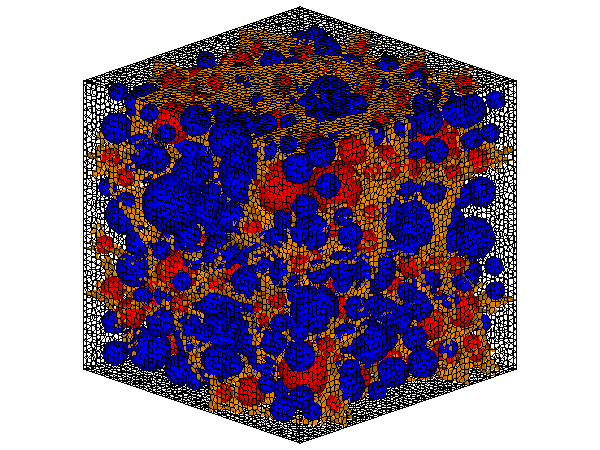
\includegraphics[width=.8\linewidth]{Files/exp_3D/ASR/A30P25_1_c.png}
    \caption{Case 1: 0.1651\% Expansion}
    \end{subfigure}
    %*******
    \begin{subfigure}{.5\textwidth}
      \centering
      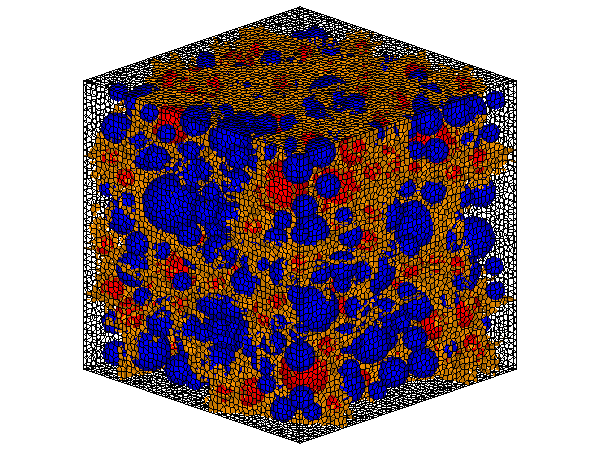
\includegraphics[width=.8\linewidth]{Files/exp_3D/ASR/A30P25_2_c.png}
    \caption{Case 2: 0.3606\% Expansion}
    \end{subfigure}%
    %*******
    \begin{subfigure}{.5\textwidth}
      \centering
      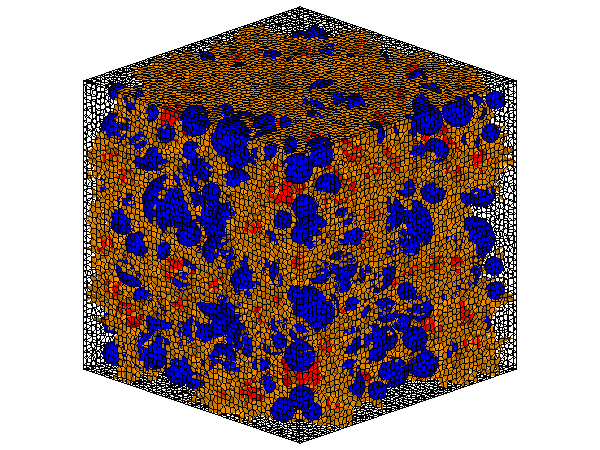
\includegraphics[width=.8\linewidth]{Files/exp_3D/ASR/A30P25_3_c.png}
    \caption{Case 3: 0.7024\% Expansion}
    \end{subfigure}
    %*******
    \begin{subfigure}{.5\textwidth}
      \centering
      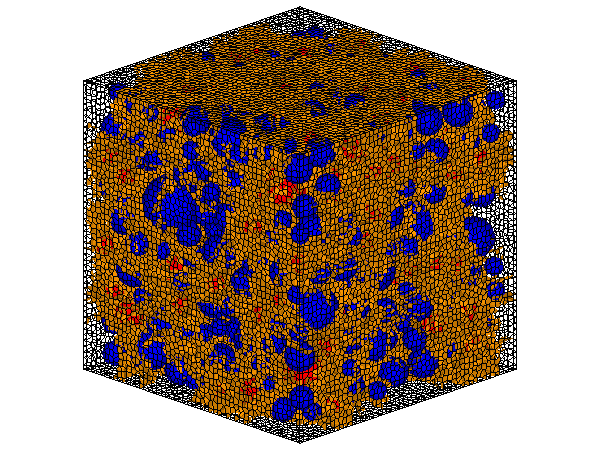
\includegraphics[width=.8\linewidth]{Files/exp_3D/ASR/A30P25_4_c.png}
    \caption{Case 4: 1.0201\% Expansion}
    \end{subfigure}%
    %*******


  \caption{3D Inner Cracks}
  \label{fig:ASR_A30P25_crack}
\end{figure}

Figure \ref{fig:ASR_A30P25_3D} and Figure \ref{fig:ASR_A30P25_3DS} show surface crack pattern after ASR expansion of 30\% coarse aggregate cases with 25\% of the coarse aggregate inside are ASR reactive. Figure \ref{fig:ASR_A30P25_crack} shows the inner crack distribution.

Here 2 cases from 25\% ASR reactive coarse aggregate in 30\% total coarse aggregate model and 75\% ASR reactive coarse aggregate in 30\% total coarse aggregate model in relatively close global expansion rate are compared to show the influence of ASR reactive coarse aggregate ratio on cracking pattern.

\begin{figure}[ht!]
\centering

    %*******
    \begin{subfigure}{.5\textwidth}
      \centering
      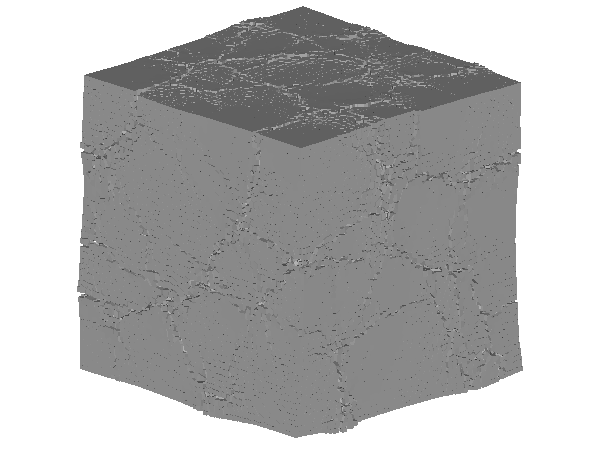
\includegraphics[width=.8\linewidth]{Files/exp_3D/ASR/A30P25_2_3d.png}
    \caption{A30P25 Case 2: 0.3606\% Expansion \\ 3D Surface Crack}
    \end{subfigure}%
    %*******
    \begin{subfigure}{.5\textwidth}
      \centering
      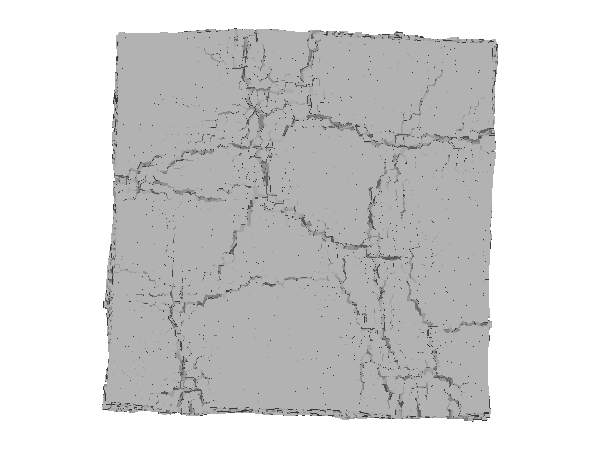
\includegraphics[width=.8\linewidth]{Files/exp_3D/ASR/A30P25_2_3ds.png}
    \caption{A30P25 Case 2: 0.3606\% Expansion \\ 3D Surface Cracks (Single Side View)}
    \end{subfigure}
    %*******
    \begin{subfigure}{.5\textwidth}
      \centering
      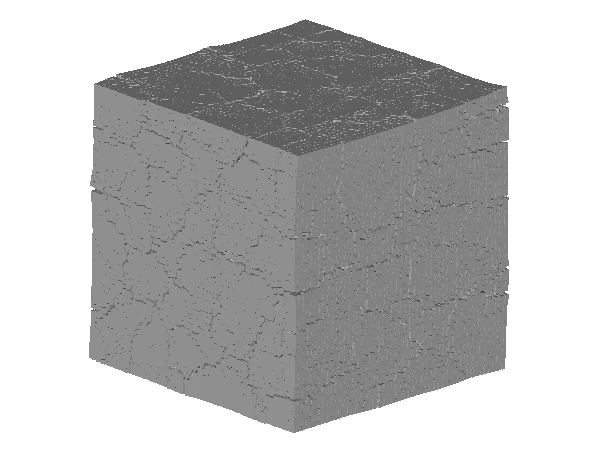
\includegraphics[width=.8\linewidth]{Files/exp_3D/ASR/A30P75_3_3d.png}
    \caption{A30P75 Case 3: 0.4223\% Expansion\\ 3D Surface Crack}
    \end{subfigure}%
    %*******
    \begin{subfigure}{.5\textwidth}
      \centering
      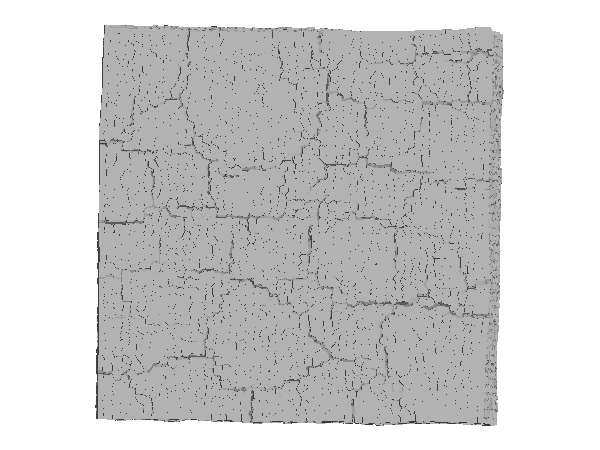
\includegraphics[width=.8\linewidth]{Files/exp_3D/ASR/A30P75_3_3ds.png}
    \caption{A30P75 Case 3: 0.4223\% Expansion\\ 3D Surface Cracks (Single Side View)}
    \end{subfigure}
    %*******

  \caption{Comparing Between A30P25 and A30P75 3D Surface Cracks ($Deformation \times 10$)}
  \label{fig:ASR_A30P25vsA30P75_3D}
\end{figure}


For the reactive aggregate ratio of 25\% model, case 2 is chosen, giving 0.002initial strain for ASR reactive interfaces in each step, and reached 0.3606\% one-dimensional expansion after 20 steps. And for the reactive aggregate ratio of 75\% model, case 3 is chosen, giving 0.001 initial strain for ASR reactive interfaces and reached 0.4223\% one-dimensional expansion after 20 steps.

\begin{figure}[ht!]
\centering

    %*******
    \begin{subfigure}{.5\textwidth}
      \centering
      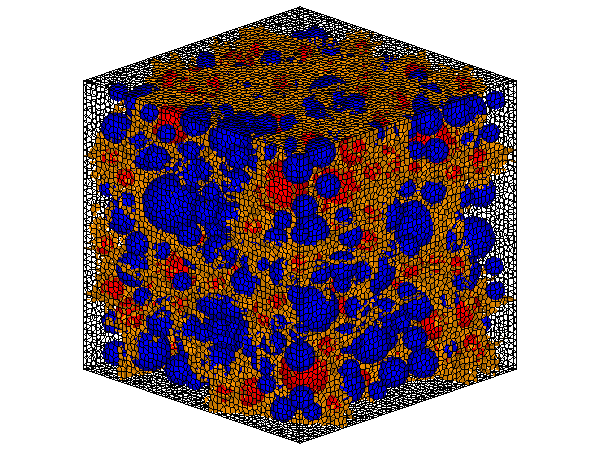
\includegraphics[width=.8\linewidth]{Files/exp_3D/ASR/A30P25_2_c.png}
    \caption{A30P25 Case 2: 0.3606\% Expansion \\ 3D Inner Crack}
    \end{subfigure}%
    %*******
    \begin{subfigure}{.5\textwidth}
      \centering
      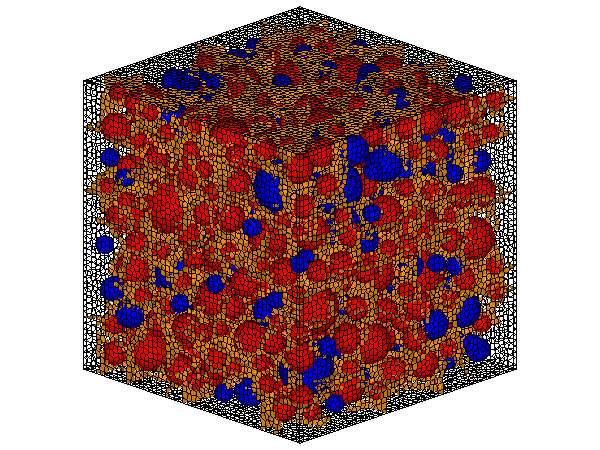
\includegraphics[width=.8\linewidth]{Files/exp_3D/ASR/A30P75_3_c.png}
    \caption{A30P75 Case 3: 0.4223\% Expansion\\ 3D Inner Crack}
    \end{subfigure}

  \caption{Comparing Between A30P25 and A30P75 3D Surface Cracks ($Deformation \times 10$)}
  \label{fig:ASR_A30P25vsA30P75_3D_crack}
\end{figure}

As can be seen in Figure \ref{fig:ASR_A30P25vsA30P75_3D}, at a relatively close global expansion ratio, the cracks are more concentrated with less reactive coarse aggregate ratio case (reactive aggregate ratio of 25\% cases here). Here inner cracking interfaces with over 0.03 mm are colored in orange. This indicated that the concentration of location generate expansion could result in the concentration of global cracking distribution, which consists with the previous cases when the total aggregate percentage is decreased.

Still, both of the cases show clear characteristic map cracking which observed in typical ASR expanded concrete structures.

And from Figure \ref{fig:ASR_A30P25vsA30P75_3D_crack}, the inner cracking distribution of 2 cases are also compared. It can be seen that the case with less reactive coarse aggregate ratio (15\% ASR reactive aggregate) is having less distributed cracks (larger than 0.03 mm).



\begin{table}[!h]
  \caption{Comparing Between A30P25 and A30P25 3D Surface Cracks}
\centering
\begin{tabular}{ ||p{4cm}|p{4cm}|p{4cm}|| }
\hline
 Crack Width [mm] &  A30P25 Case 2 Total Cracked Interfaces &  A30P75 Case 3 Total Cracked Interfaces \\
 \hline\hline

   0.00000 - 0.00005 & 327828 & 316744 \\
   0.00005 - 0.00010 & 280821 & 286704 \\
   0.00010 - 0.00020 & 256125 & 263943 \\
   0.00020 - 0.00050 & 229235 & 234672 \\
   0.00050 - 0.00100 & 189533 & 183238 \\
   0.00100 - 0.00300 & 154639 & 131553 \\
   0.00300 - 0.01000 & 85126 & 42432 \\
   0.01000 - 0.03000 & 6584 & 275 \\
   0.03000 - 0.10000 & 0 & 0 \\
   0.1000+ & 0 & 0 \\

  \hline
  \end{tabular}

\label{table:A30P25_2_vsA30P75_3_Cracks}
\end{table}

When numerically comparing their crack distribution summarised by its crack width (Table \ref{table:A30P25_2_vsA30P75_3_Cracks}),  it can be seen that cracking face number of larger cracks the case with 25\% ASR reactive coarse aggregate is significantly higher, even when the global expansion ratio in 25\% ASR reactive coarse aggregate is slightly smaller than 75\% ASR reactive coarse aggregate case.

For the number of cracked interfaces larger than 0.003 mm, 25\% ASR reactive coarse aggregate case is 2.15 times of 75\% ASR reactive coarse aggregate case. And for the number of cracked interfaces larger than 0.01 mm, 25\% ASR reactive coarse aggregate case is 23.94 times of 75\% ASR reactive coarse aggregate case.

This significant difference in crack distribution indicates consisit with the global cracking patterns, suggest severe damage when considering the deterioration of the concrete structure.
